%===========================================================================
%	VI. Solution Evaluation
%===========================================================================

The following evaluation is expected to provide insights whether the solution works as intended during implementation. A focus is set on the testing capabilities of the \ac{cicd} pipeline in order to find potential limitations of the solution and discuss possible improvement techniques in theory. Throughout the evaluation, DataOps is compared to DevOps while focussing on the \ac{cicd} process and its testing features. This ultimately includes bottlenecks that cannot be covered by automated measures of the pipeline but rather need to be handled via conventions and best practices.

\section{Workflow Demonstration}
First of all, it might be valuable to evaluate the basic functionality of the \ac{cicd} pipeline, including its testing and deployment capabilities when no errors occur. For this matter, the general development workflow is applied. Before the following changes, the latest production-grade image was tagged with the commit ID \texttt{3c75dd5} inside \ac{ecr}.

A developer makes an arbitrary change to the Conversion Stage source code of the solution that is expected not to break the solution. This change is made in a separate feature branch of the \ac{vcs}. The developer can verify this fact by running the preexisting, automated tests locally on the developer sandbox. Then, a pull request is filed with the goal to merge the feature branch with the \texttt{master} branch, resulting in the new source code version being deployed into production. The pull request needs to include the appropriate GitHub labels, marking that the pull request should be treated as a new feature inside the Conversion \ac{cicd} pipeline. The filing could look like the screenshot provided in Figure \ref{fig:6-pr}. A pull request description is well-desired but omitted here for the sake of simplicity.
\newpage
\begin{figure}[h!]
	\centering
	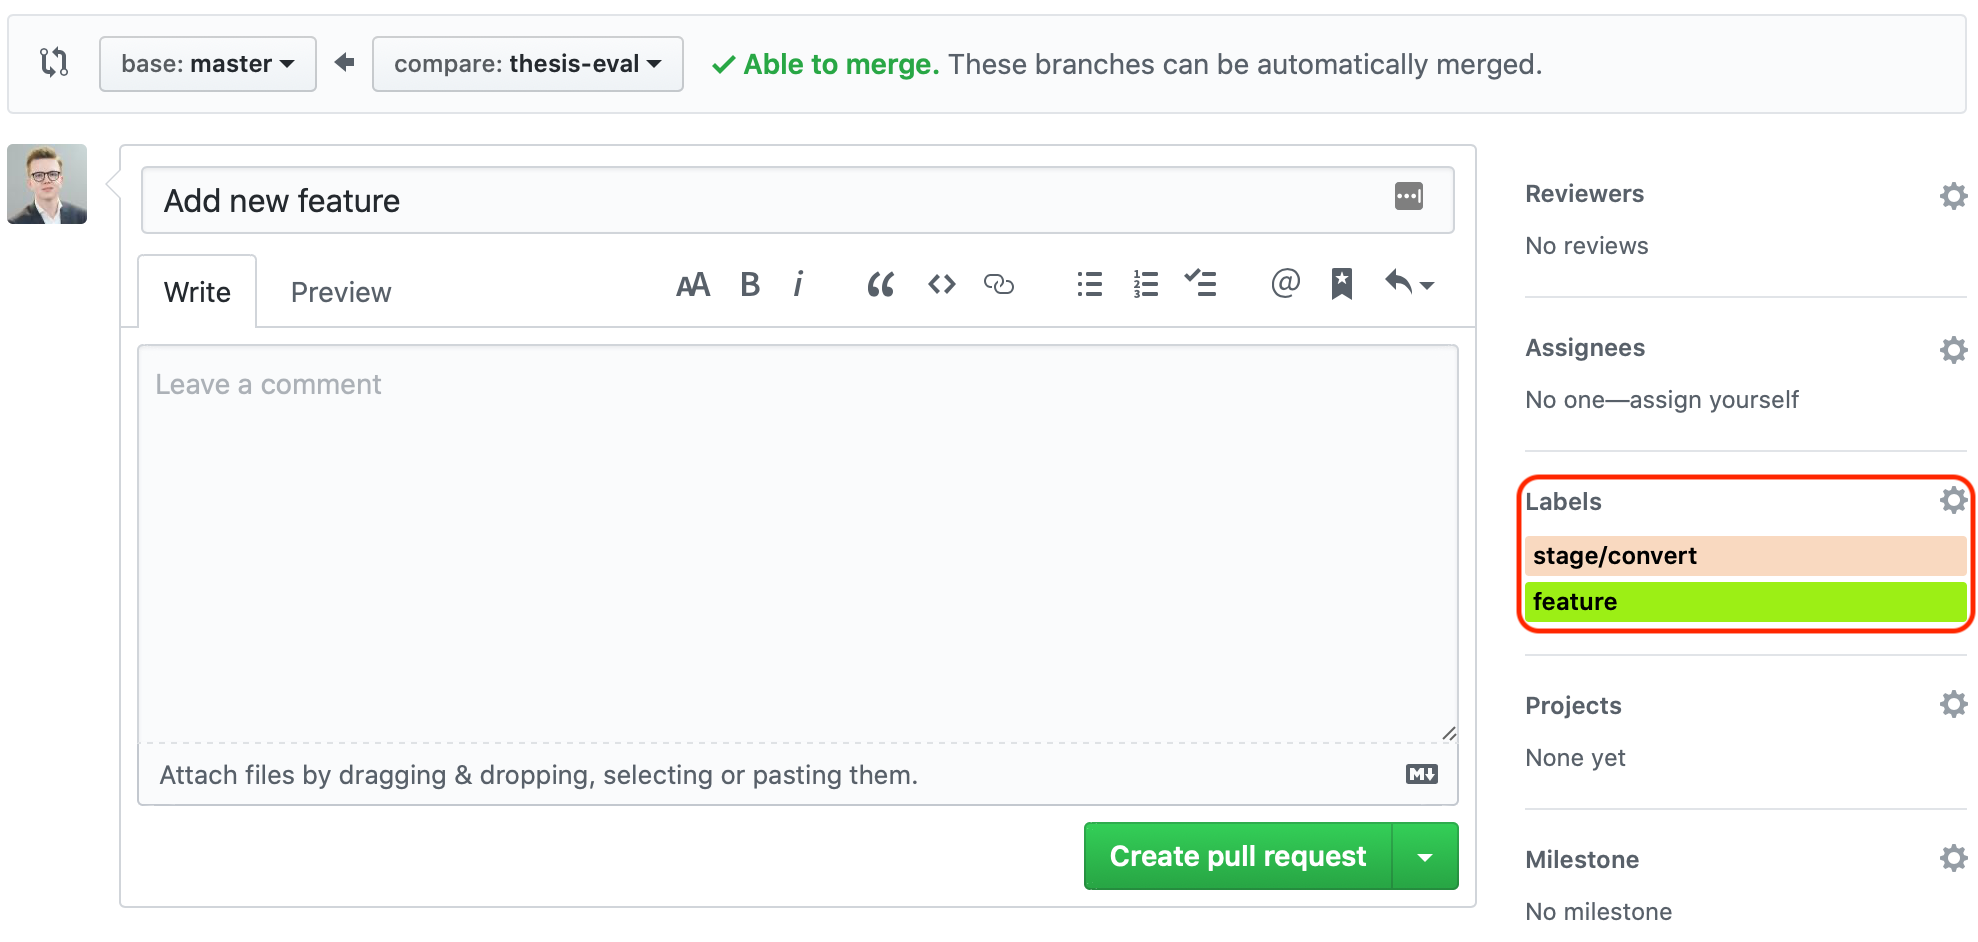
\includegraphics[width=\linewidth]{main-matter/img/6-pr.png}
	\caption{GitHub Feature Pull Request for Conversion Stage (Screenshot)}
	\label{fig:6-pr}	
\end{figure}

The first minor issue can be found inside this workflow. The developer in charge of this pull request is required to set the appropriate labels. The \texttt{feature} label missing would cause the \ac{cicd} pipeline not to run. The same applies to the stage specification label. An incorrect label could cause even more problems since this would trigger another pipeline with this stage source code, resulting in the build phase failing. The problem could be resolved by splitting up the repositories by stage but would remove the overall availability of the entire project's source code. This could have a negative impact on the productivity of the teams working on the project.

In case of correctly chosen labels, the Conversion Stage pipeline is triggered. A new pull request is automatically added to Jenkins and can be seen in the corresponding overview of the Jenkins \acs{ui}, shown in the screenshot in Figure \ref{fig:6-jenkins-pr}.

\begin{figure}[h!]
	\centering
	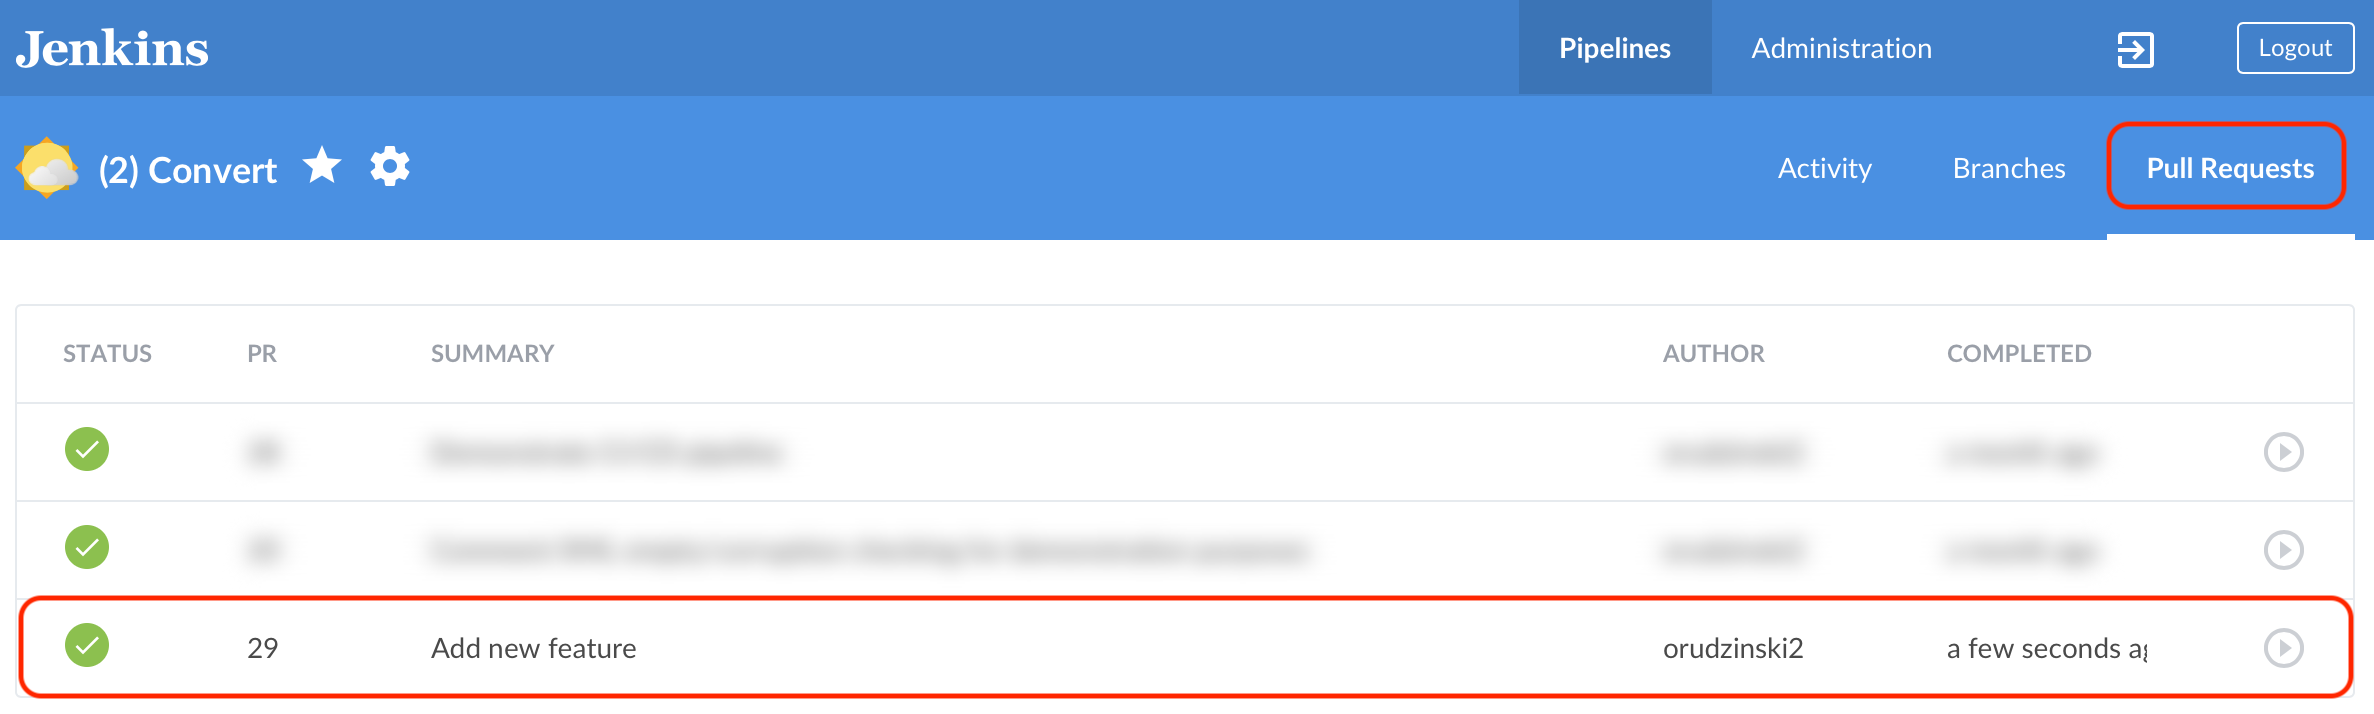
\includegraphics[width=\linewidth]{main-matter/img/6-jenkins-pr}
	\caption{Pull Request in Jenkins \acs{ui} (Screenshot)}
	\label{fig:6-jenkins-pr}
\end{figure}

The green checkmark shows that the pull request was evaluated, successfully verified and deployed. The specific pipeline overview can be retrieved by inspecting the corresponding pull request. This yields the following screenshot in Figure \ref{fig:6-jenkins-job-success}.

\begin{figure}[h!]
	\centering
	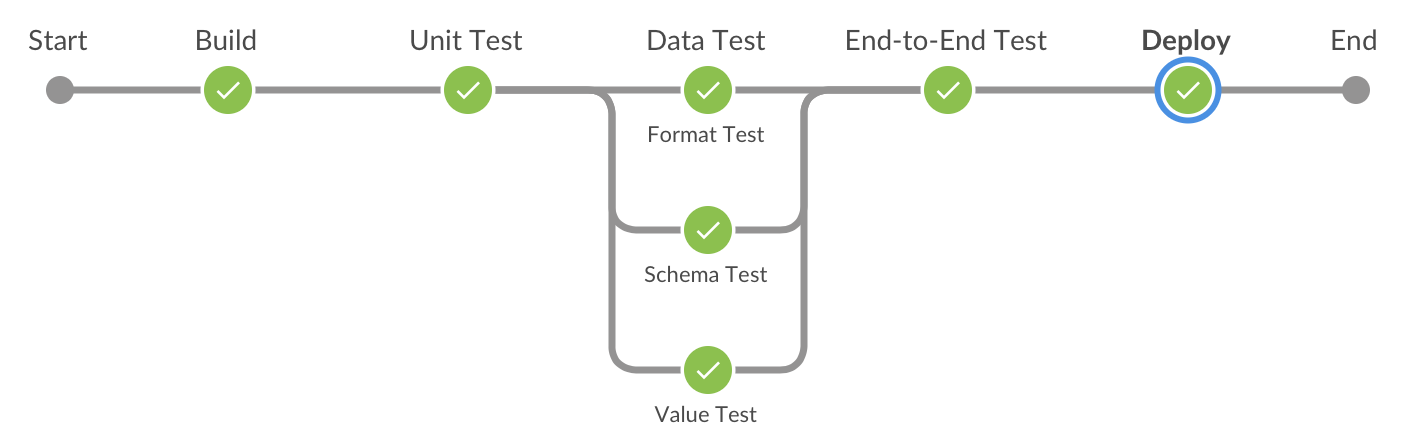
\includegraphics[width=\linewidth]{main-matter/img/6-jenkins-job-success}
	\caption{Successful Pipeline Job in Jenkins \acs{ui} (Screenshot)}
	\label{fig:6-jenkins-job-success}
\end{figure}

Since the deployment has run through correctly, \ac{ecr} should have received a new image. This image should be tagged with the last commit ID of the pull request as well as the \texttt{latest} tag. Inspecting the corresponding repository inside the \ac{aws} Console verifies this claim, presented in the screenshot of Figure \ref{fig:6-ecr}

\begin{figure}[h!]
	\centering
	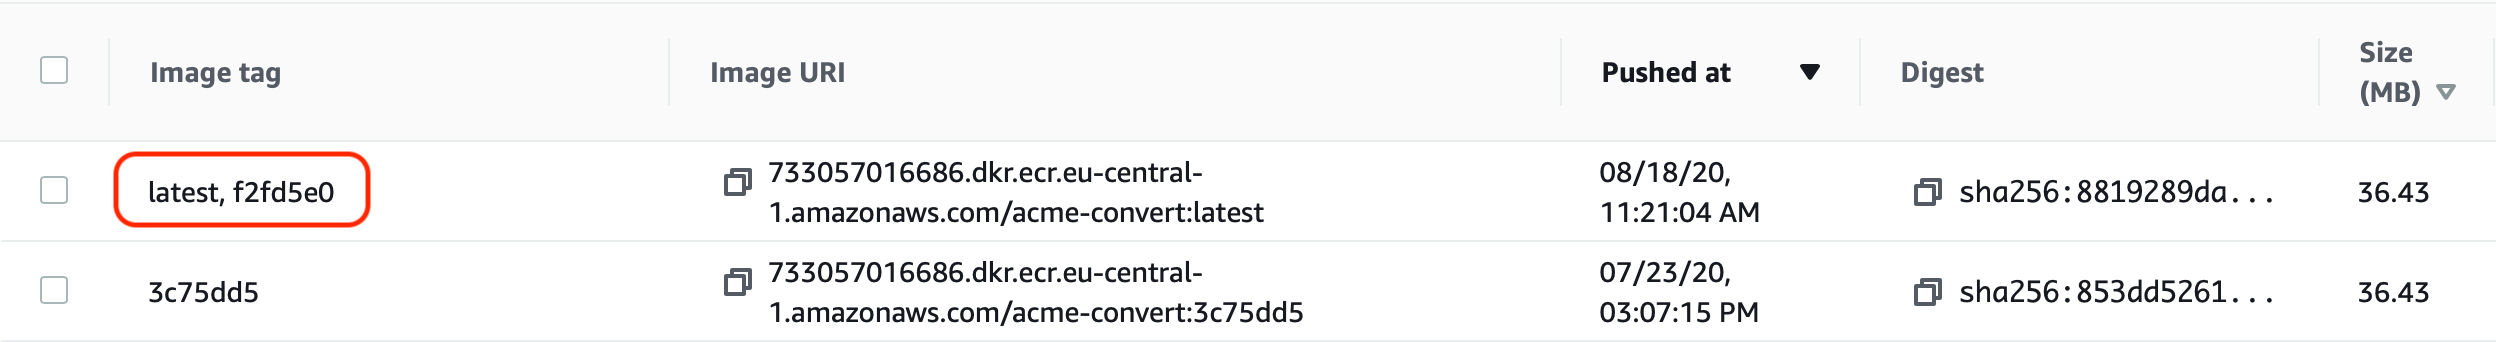
\includegraphics[width=\linewidth]{main-matter/img/6-ecr}
	\caption{Image List of the Conversion Stage \acs{aws} \ac{ecr} Repository (Screenshot)}
	\label{fig:6-ecr}
\end{figure}

It can be seen, that the new image has been included with the appropriate tags. The old version of the image still resides in the repository for versioning reasons. Because of the correct tagging, Airflow will use this updated version of the Conversion Stage image for upcoming analyses. 

The source code change is not reflected in the GitHub repository, yet. The feature branch still exists and the \texttt{master} branch has not been changed. Since the required \ac{cicd} checks have run through successfully, the developer can now merge the feature branch with the \texttt{master} branch. This manual procedure is required by GitHub. This can be seen as another issue of lacking automation since the developer may not forget to merge the branches and remove the feature branch after the deployment has been conducted successfully. Existing copies of the previous \texttt{master} branch inside other development sandboxes need to be updated now since working with the outdated version might cause compatibility issues of upcoming versions as well as so-called \textit{merge conflicts} within GitHub, where the feature might be correct by means of the \ac{cicd} evaluation, but the code history of the branches to merge does not allow for an automatic merge and requires manual correcting.

At this point, one iteration of the \ac{cicd} workflow is completed.

\section{Testing Capability Evaluation}
The previous evaluation use case did not contain on purpose in order to demonstrate the desired development workflow. Now, the workflow of the pipeline is evaluated for different kinds of issues. In general, this is divided into two categories:

\begin{enumerate}
	\item issues that result from updating existing features, and
	\item issues that result from creating new features.
\end{enumerate}

\subsection{Feature Update Testing}
The most na\"ive approach is to remove a line of code that is required by the testing framework. This simulation is comparable to a scenario where an existing feature is updated but a required functionality was removed. The testing framework is supposed to be invoked by the \ac{cicd} pipeline job and catch the issue. Specifically, the line checking for a corrupted \ac{xml} file inside the analytics script of the Conversion Stage is removed. This data handling function has been presented in Section \ref{sec:5-3-3-2}.

The process of filing a pull request remains identical. Jenkins' pull request job is triggered again, resulting in the job workflow depicted in the screenshot in Figure \ref{fig:6-jenkins-pr-fail1}.

\begin{figure}[h!]
	\centering
	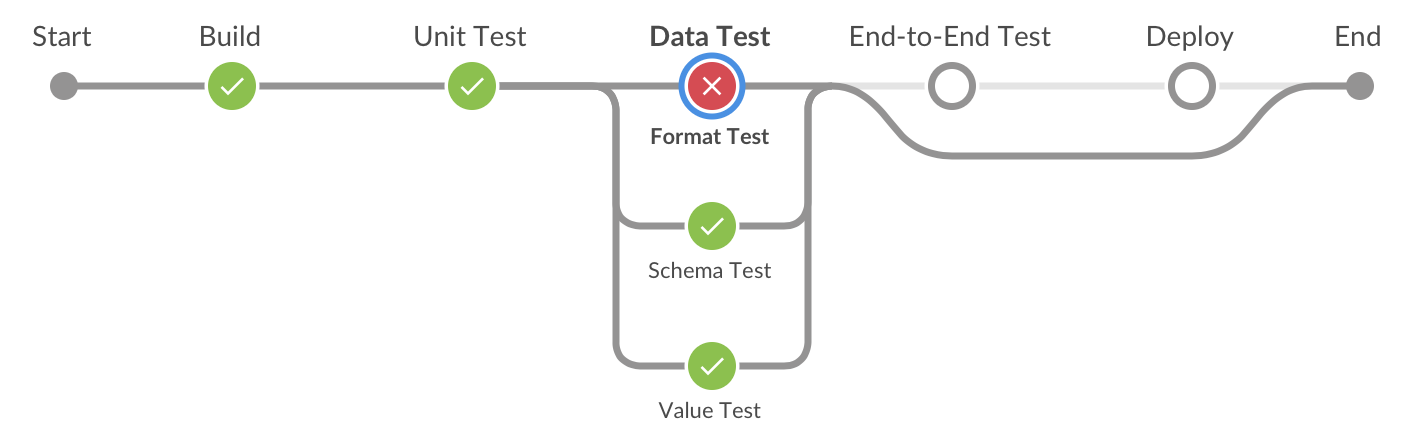
\includegraphics[width=\linewidth]{main-matter/img/6-jenkins-pr-fail1}
	\caption{Failing Pipeline Job in Jenkins \acs{ui} (Line Missing) (Screenshot)}
	\label{fig:6-jenkins-pr-fail1}
\end{figure}

Since \ac{xml} corruption testing is subject to the data format testing suite, the corresponding stage inside the \ac{cicd} pipeline fails. The upcoming stages are skipped such that no flawed deployment is conducted. The \textit{Tests} tab of the job inside the Jenkins \ac{ui} provides insights to the tests that have been run during the testing stages and highlights tests that did not pass. This overview is shown in a screenshot in Figure \ref{fig:6-jenkins-tests}.
\newpage
\begin{figure}[h!]
	\centering
	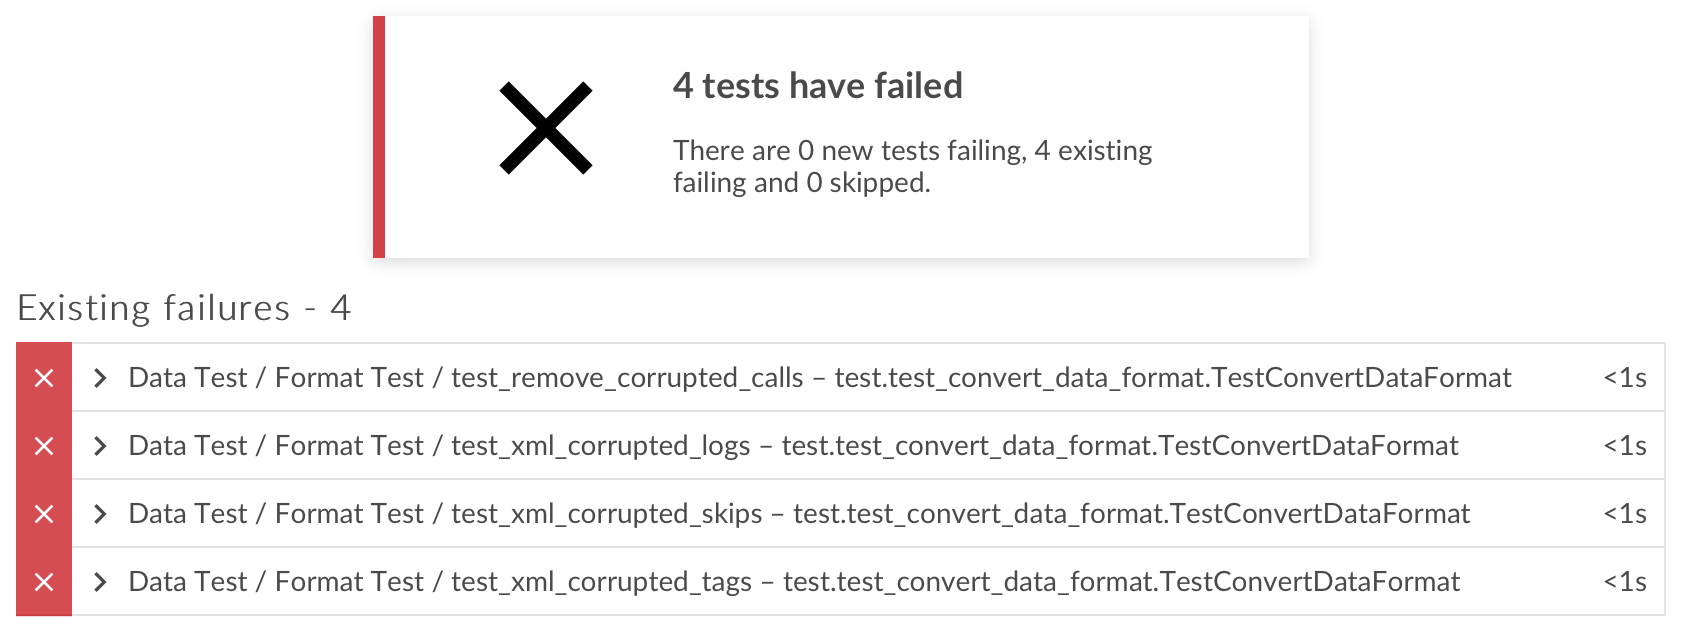
\includegraphics[width=\linewidth]{main-matter/img/6-jenkins-tests}
	\caption{Failing Tests in Jenkins \acs{ui} (Line Missing) (Screenshot)}
	\label{fig:6-jenkins-tests}
\end{figure}

It can be seen that all tests regarding \ac{xml} corruption fail. This is because the centralized \texttt{remove\_corrupted(...)} data handling function is not called inside the analytics script anymore. Since all handling measures are defined in that function, no measure is actually taken when the function call is missing. In case of the data handling function missing individual handling steps, the corresponding tests would fail. These test results are meant to provide valuable insights to the developer. The developer can analyze the problem, fix occurrences, and push a new commit to the pull request. When the test failures have been resolved, the updated version can be correctly deployed.

Similar failure detections occur with different changes of the source code. This shows that the pipeline is capable of stopping a deployment process based on the existing tests. This requires the assumption that all tests suites are complete and perform as expected.

\subsection{Feature Creation Testing}
The previous paragraphs covered the integration of an already existing feature. The following paragraphs deal with the creation and adequate testing of a new feature. The consideration of this practical area is important since the solution at hand can encounter changing requirements that need to be embodied accordingly.

For this evaluation, assume that the product owner of the \ac{mba} data pipeline requests a new feature that includes the weather data of the creation date of the purchase information to the analysis. This could be used to find a possible correlation between the purchasing behavior of the retail company's customers and the weather situation at the given point in time. The development teams find that the integration of weather data is mostly suited to be developed inside the Conversion Stage of the data pipeline since it represents the first stage that has access to the raw purchasing data.

The na\"ive implementation of that feature is shown in Source Code Excerpt \ref{src:6-weather} below.

\begin{listing}[h!]
	\inputminted{python}{main-matter/src/6-weather.py}
	\caption{Na\"ive Implementation of a Weather Data Integration Feature}
	\label{src:6-weather}
\end{listing}

The feature's corresponding function is placed right after the reformatting of the \ac{pos}Log dictionaries and, thus, right before the \ac{json} file export. For each purchase, the weather that corresponds to the transaction date and place is requested from an external weather \acs{api} (ll. 5--12). For simplicity reasons, the average weather data in degrees Celsius is extracted (ll. 14--16) and added to the dictionary (l. 18). There are multiple issues that can occur when such a code fragment is integrated to the solution. 

\subsubsection{Feature Testing Limitations}
When performing an update of an existing feature, the validation of the update can be conducted by running the preexisting tests of the corresponding feature. However, the development of a new feature also means writing new tests. The \ac{cicd} pipeline can only stop a feature from being deployed into production when corresponding feature tests fail. In case that these tests do not exist, the \ac{cicd} pipeline cannot recognize any issues and publishes an untested feature. This situation is highly undesired and problematic for the integrity of such a solution. Plus, it yields discussions that go beyond the technical aspects of data analytics development but need to deal with the developer's understanding and acceptance of an agile development workflow.

In agile development, a developer is always in charge of testing the feature that he or she works on \cite[18]{Kaiser}. Principles like \ac{tdd} have been introduced to support the importance of the testing process \cite[1]{Karac2018}. DataOps testing principles might develop this into a data-driven approach (i.e., test data first, then solution test, then feature implementation). Nevertheless, from a general point of view, these principles can be suggested or required by convention, but not technically enforced. A separate tool could evaluate if tests exist for a given feature by executing all test suites and calculating the feature's occurrences in these tests. This measurement is referred to as the \textit{test code coverage} \cite[15]{Garrett2011}. However, such a mechanism could be bypassed by simply executing a function inside a test case. This could presume the feature being tested and allow the change to be deployed into production. Other, more complex metrics (e.g., defect fix retest, test effectiveness, etc. \cite[15]{Garrett2011}) could be suited for more in-depth testing quality assurance, but would still be required to be implemented and reevaluated for the given use cases over time.  All in all, DataOps requires the acceptance and consciousness of agile processes and does not only rely on technical measurements to control their fulfillment.

Even with appropriate testing, the issue is still present. This is because the feature and the corresponding tests are conducted by human developers. The person behind a feature might have a different understanding of the feature than the product owner or simply miss an edge case during testing that could lead to further issues. Specifically, the developer might implement the feature to provide weather data in degrees Fahrenheit and test the value correctness accordingly. The product owner or other developers might expect degrees Celsius instead. As with pure software development, such a feature change also requires updating the solution requirements and general collaboration and communication between developers and development teams of the separate stages. In general, all contributors should have the same understanding of a feature in order to prevent inconsistencies.

This issue also introduces the discussion of \textit{testing tests} that are meant to test the functionality of the source code. The addition of testing validation based on previously mentioned complex testing quality metrics might mean more effort. With these validation systems, the question behind \textit{their} validity can be posed and the discussion continues. This ultimately means that automated tests might not suffice for confident and correct deployment of such a solution. Apart from that, peer code reviews and other interdisciplinary measures might need to be taken in order to rule out mistakes that cannot be uncovered by traditional software solution testing.

\subsubsection{Importance of Regression Testing}
Another issue can be found in regression. Assume that a previous \ac{mba} needs to be re-conducted because an error inside its values is suspected. The data from the target \ac{mba} originates from a time before this feature was requested. The previous \ac{mba} did also not consider weather data for its analysis. When the analysis is repeated, the \ac{mba} might, purposefully, yield different results. However, this behavior is not desired. The addition of a new feature may not lead to inconsistencies between two versions of the same analysis. This would create a new data quality issue and result in further issues in the upcoming analytical stages. Instead, this feature may only be used for new analyses (e.g. by specifying a minimum date that needs to be present in the input data). This behavior correctness needs to be ensured by including a corresponding test to the testing suite of the solution.

Another form of regression testing in this case is the execution of previous tests. Their passing will ensure that the new feature does not change the behavior of previously existing features. Since this feature only adds an attribute to the output of the stage, the previous features and feature tests run correctly. Other feature implementations might require the change of preexisting features which then might require the adaptation of the corresponding tests, etc. \\\

All in all, the general testing process, including its limitations and technical bottlenecks, can be compared to agile DevOps testing. On the other hand, regression testing plays a priority role in data analytics testing and needs to be taken into account for each feature. This finding preliminarily corresponds with the hypothesis from Section \ref{sec:2-2-innovation-pipeline}. Currently, it can be said that the DataOps testing process is similar to DevOps, but takes data-specific requirements into account.

\section{Impact Analysis of Different Testing Levels}
In order to evaluate further potential differences to the DevOps testing process, the following section deals with the different testing levels (unit, integration, and end-to-end testing) in the \ac{mba} DataOps pipeline environment. This part of the evaluation is expected to yield insights about the specific impact of the testing levels in such a data-driven environment, built up in a highly externalized technical infrastructure. 

This evaluation is conducted based on testing use cases that occur at different hierarchical levels of the testing process. These use cases are not explicitly tested for by the solution. The evaluation will provide information on how insightful the error recognition of the different testing levels is for recovering from the problem. The use cases are described as follows:

\begin{description}
	\item[Non-Existing \ac{s3} Bucket \acs{uri} Provided] The format of the \ac{uri} is correct, but the bucket does not exist (typographic error, deprecated bucket reference, etc.).
	\item[Invalid \ac{aws} \ac{iam} Credentials Provided] The format of the \ac{iam} credential key pair is correct, but it either does not provide sufficient access to the resources, or it is deprecated .
	\item[Container Task Ran Out of Memory] The container that an analytics stage is run in cannot finish its job because it requires more memory than expected.
\end{description}

\subsection{Failure Case Execution}
These cases are designed and invoked, leading to the following results:

\subsubsection{Non-Existing \ac{s3} Bucket \acs{uri} Provided}
\begin{table}[h!]
\centering
\begin{tabular}{r!{\vrule width 1pt}l|l|l}
\multicolumn{4}{c}{\textbf{Non-Existing \acs{s3} Bucket \acs{uri} Provided}}                                                                        \\[0.4em] \ChangeRT{1pt}
\makecell[r]{\textbf{Level}}       & \textbf{Unit} & \textbf{Integration}                                                       & \textbf{End-to-End} \\ \ChangeRT{1pt}
\makecell[r]{\textbf{Result}}      & \cellcolor{green!25}passed        & \cellcolor{red!25}failed                                                                     & \cellcolor{gray!25}\textit{skipped}                \\ \hline
\makecell[r]{\textbf{Information}} &               & \makecell[l]{\texttt{boto3} Exception:\\ \texttt{404 Not Found}} &                    
\end{tabular}
\caption{Testing Evaluation: Non-Existing \acs{s3} Bucket \acs{uri} Provided}
\label{tab:6-bad-s3}
\end{table}

As can be seen in Table \ref{tab:6-bad-s3}, the corresponding unit test only tests if \ac{s3} \acsp{uri} of incorrect format are caught and reported. Since the \acs{uri} at hand is correct, the unit test passes. The integration (data) test actually connects to the bucket, resulting in an \texttt{boto3} exception, reporting that the provided \ac{s3} bucket does not exist.

The process of mocking the \ac{s3} connection service inside the unit test would not have helped here since the actual existence of the infrastructure can only be evaluated within the scope of the infrastructure.
\newpage
\subsubsection{Invalid \ac{aws} \ac{iam} Credentials Provided}
\begin{table}[h!]
\centering
\begin{tabular}{r!{\vrule width 1pt}l|l|l}
\multicolumn{4}{c}{\textbf{Invalid \ac{aws} \ac{iam} Credentials Provided}}                                                                        \\[0.4em] \ChangeRT{1pt}
\makecell[r]{\textbf{Level}}       & \textbf{Unit} & \textbf{Integration}                                                       & \textbf{End-to-End} \\ \ChangeRT{1pt}
\makecell[r]{\textbf{Result}}      & \cellcolor{green!25}passed        & \cellcolor{red!25}failed                                                                     & \cellcolor{gray!25}\textit{skipped}                \\ \hline
\makecell[r]{\textbf{Information}} &               & \makecell[l]{\texttt{boto3} Exception:\\ \texttt{Access Denied}} &                    
\end{tabular}
\caption{Testing Evaluation: Invalid \ac{aws} \ac{iam} Credentials Provided}
\label{tab:6-bad-iam}
\end{table}
This case is similar to the incorrect \acs{uri} and results in the same test outcome, shown in Table \ref{tab:6-bad-iam}. Only the infrastructure itself can evaluate the credentials and report an issue. This is why, again, the unit test passes, while the integration test results in another exception, mentioning that the provided credentials cannot be used for the current operation.

\subsubsection{\acs{ecs} Container Task Ran Out of Memory}
\begin{table}[h!]
\centering
\begin{tabular}{r!{\vrule width 1pt}l|l|l}
\multicolumn{4}{c}{\textbf{\acs{ecs} Container Task Ran Out of Memory}}                                                                        \\[0.4em] \ChangeRT{1pt}
\makecell[r]{\textbf{Level}}       & \textbf{Unit} & \textbf{Integration}                                                       & \textbf{End-to-End} \\ \ChangeRT{1pt}
\makecell[r]{\textbf{Result}}      & \cellcolor{green!25}passed        & \cellcolor{green!25}passed                                                                     & \cellcolor{red!25}failed                \\ \hline
\makecell[r]{\textbf{Information}} &               &  & \makecell[l]{\texttt{boto3} Exception:\\ \texttt{OutOfMemoryError: Container killed}\\\texttt{due to memory usage}}                  
\end{tabular}
\caption{Testing Evaluation: \acs{ecs} Container Task Ran Out of Memory}
\label{tab:6-oom}
\end{table}
In this case, both the unit and integration tests do not recognize the problem. Only the end-to-end test provides the information that the corresponding \ac{ecs} task has failed because of lacking memory capacity, shown in Table \ref{tab:6-oom} This is because the integration tests are performed in containerized environments on the Jenkins server instance. These Docker containers do not have any resource limitations \cite{docker}, other than the \ac{ecs} tasks that require performance specifications in their definitions. Only the end-to-end test makes use of this infrastructural service inside the solution.

\subsection{Testing Impact Evaluation}
The presented use cases yield a number of insights. First, the typical, DevOps-inspired testing level hierarchy and its degrees of testing isolation do not hold in an environment that is mostly created out of external resources. The cloud-driven infrastructure cannot be taken into account by unit tests since these are supposed to neglect these aspect and purely focus on the feature under test. When the infrastructure access is a crucial component of the feature, the unit test cannot recognize any issues.

Another aspect that follows is the strict separation of the testing levels. Taking the findings of the failure use cases into account, all infrastructure-related testing might be conducted during integration testing. This could also include \acs{uri} and \acs{iam} credential format tests that do not require infrastructure access but categorically fit inside the same testing suite. This aspect has partly been considered during development: certain data handling function tests could have been created in the domain of granular unit tests. Since their overall features relate to the data-driven part of the solution, which has been tested during integration testing, the remaining tests are performed similarly.

Finally, the last failure use case that was only recognized by end-to-end testing opens up another discussion topic. In general, the performance measures could have been implemented into the integration testing level that makes use of Jenkins-driven Docker containers. This would require additional testing effort and, potentially, the redesign of the deployment structure within the \ac{cicd} pipeline. While the overall reason behind testing should be the validation of feature functionality, strictly focussing on the definition of the testing levels could increase time and cost inside the development process.

As emphasized throughout this entire work, DataOps use cases and their corresponding automation and testing designs highly differ depending on the solution requirements, data governance definitions, etc. For the \ac{mba} data pipeline, unit tests provide little value to the actual testing expressiveness. There exists a general discussion questioning the value of unit tests \cite{Coplien}\cite{Golub2020}. This finding goes hand-in-hand with this discussion. The unit test cases might be included into the integration testing area and de-granularized for potentially better testing productivity. Further evaluation could give more insights on the impact differences between integration and end-to-end testing, leading to a generally more specialized, efficient and less tradition-driven testing architecture. Nevertheless, it is proposed that DataOps tests are categorized semantically regarding their meaning for the solution rather than focussing on testing level syntax.

In generalization and comparison to the DevOps testing process, it can still be said that automated testing is performed inside its designated steps inside the \ac{cicd} process prior to deployment. However, data analytics solutions often have to deal with externalized services, that cannot be neglected during testing. Instead of sticking to the traditional testing pyramid, each solutions' architecture needs to be evaluated from a testability point of view in order to create a well-suited testing framework inside the DataOps use case.



